%% V0.1
%% 2020/10/09
%% by Markus Goetz

\documentclass[aspectratio=1610]{beamer}

\usepackage{helmholtzai}

\title{My Awesome ML}
\subtitle{a test of time}
\author{Susanne Doe}
\date{YYYY-MM-DD}
\institute{Insitute of Things}

\begin{document}

\maketitle

\begin{frame}
    \frametitle{Single Title}
    
    \begin{itemize}
        \item Suppose $a$
        \item Also note b
    \end{itemize}
\end{frame}

\begin{frame}
    \frametitle{Slide title}
    \framesubtitle{\textbf{Subtitle} and \emph{more}}
    
    \begin{itemize}
        \item Suppose $a$
        \item Also note b
        \begin{itemize}
            \item This entails
            \item Remember also
            \begin{itemize}
                \item I almost forgot
                \item Envision
            \end{itemize}
        \end{itemize}
    \end{itemize}
\end{frame}


\begin{frame}
\frametitle{Equations}

    \begin{equation*}
        f(x) = \sum_i wx_i^2 + \frac{\beta}{2}
    \end{equation*}
\end{frame}


\begin{frame}
    \frametitle{Columns and Figures}

    \begin{columns}
        \begin{column}{0.4\textwidth}
            \begin{enumerate}
                \item Consider A
                \item ... do not forget B
            \end{enumerate}
        \end{column}
        \begin{column}{0.4\textwidth}
            \centering
            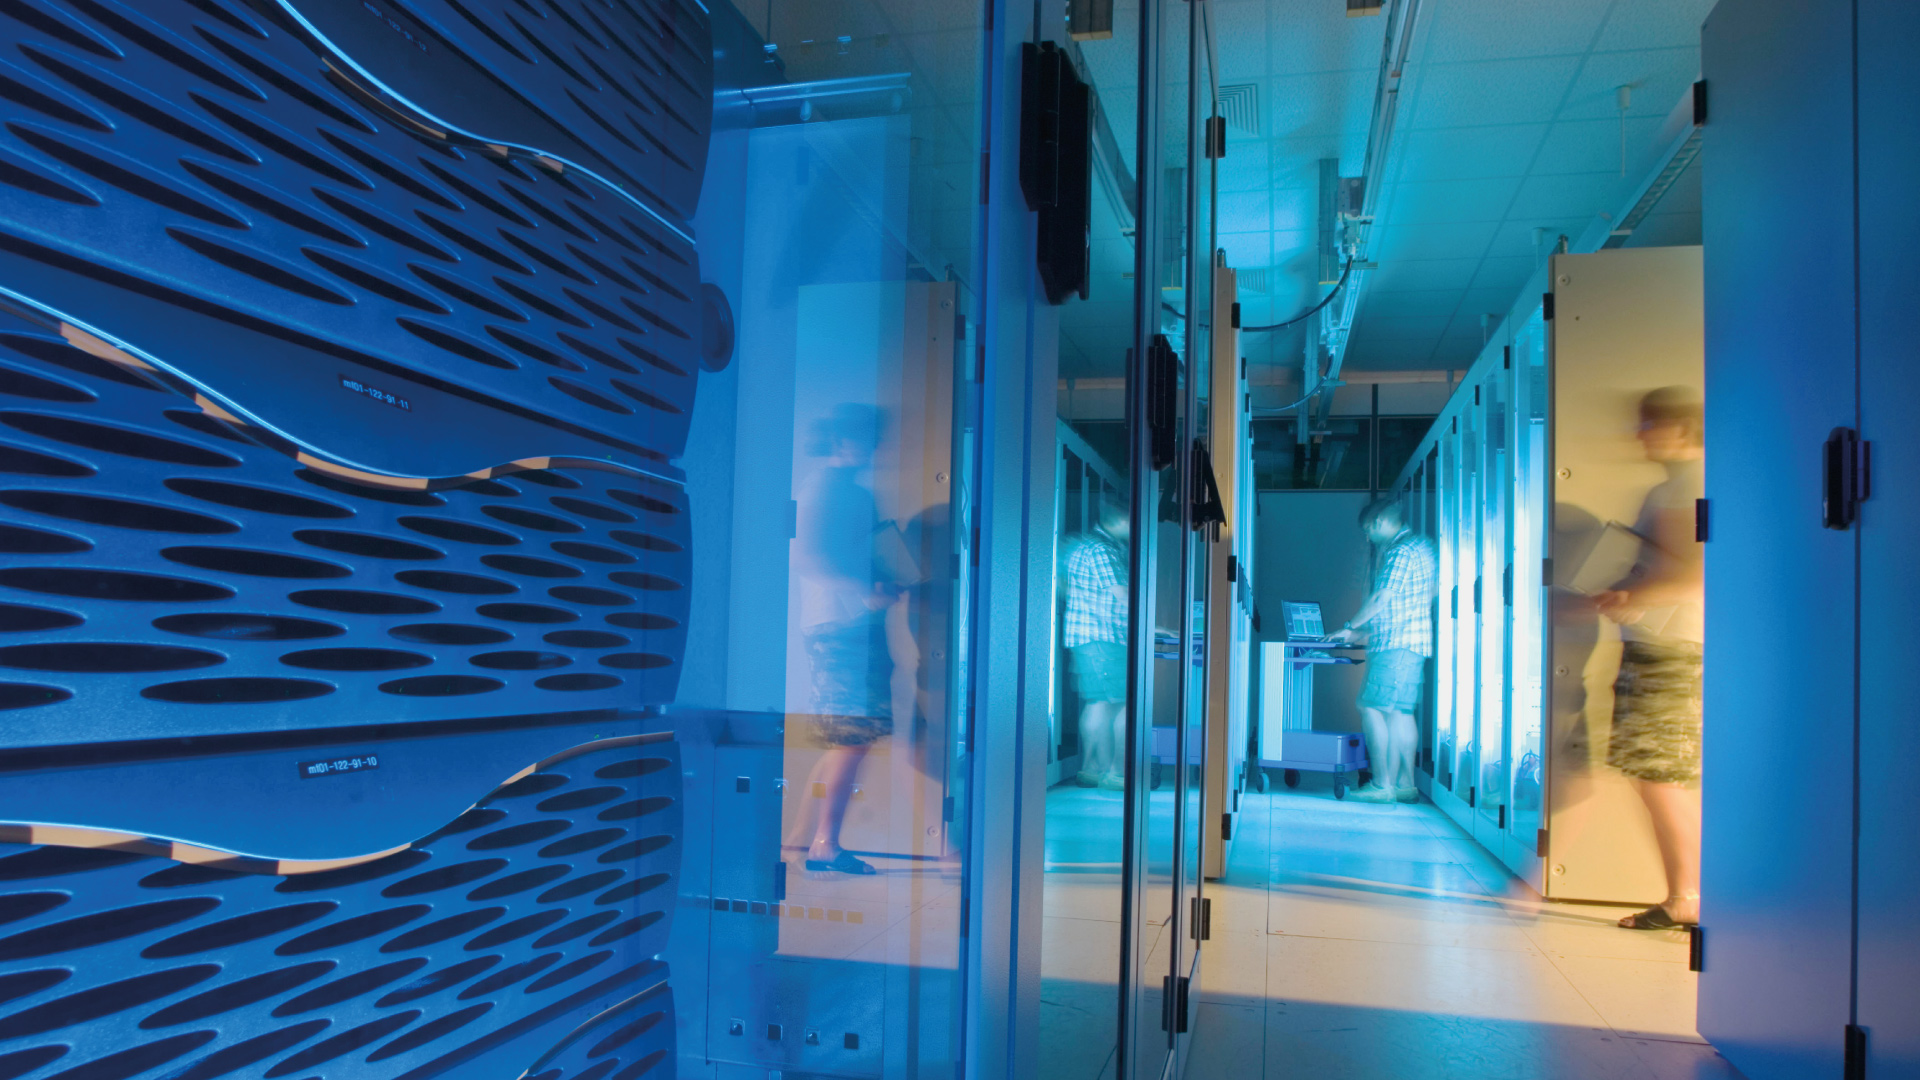
\includegraphics[width=\textwidth]{logos/hgf_key_technologies.jpg}
        \end{column}
    \end{columns}
\end{frame}

\begin{frame}[fragile]
    \frametitle{Code}
    
    \emph{Note the [fragile] specifier next to frame and the code indentation.}
    
\begin{lstlisting}[language=Python]
import numpy as np

def foo(a, b):
    """
    asd
    """
    return a + b + 1
\end{lstlisting}
\end{frame}

\section{Sections look like this}

\end{document}
